% Created by tikzDevice version 0.10.1 on 2017-09-05 18:20:56
% !TEX encoding = UTF-8 Unicode
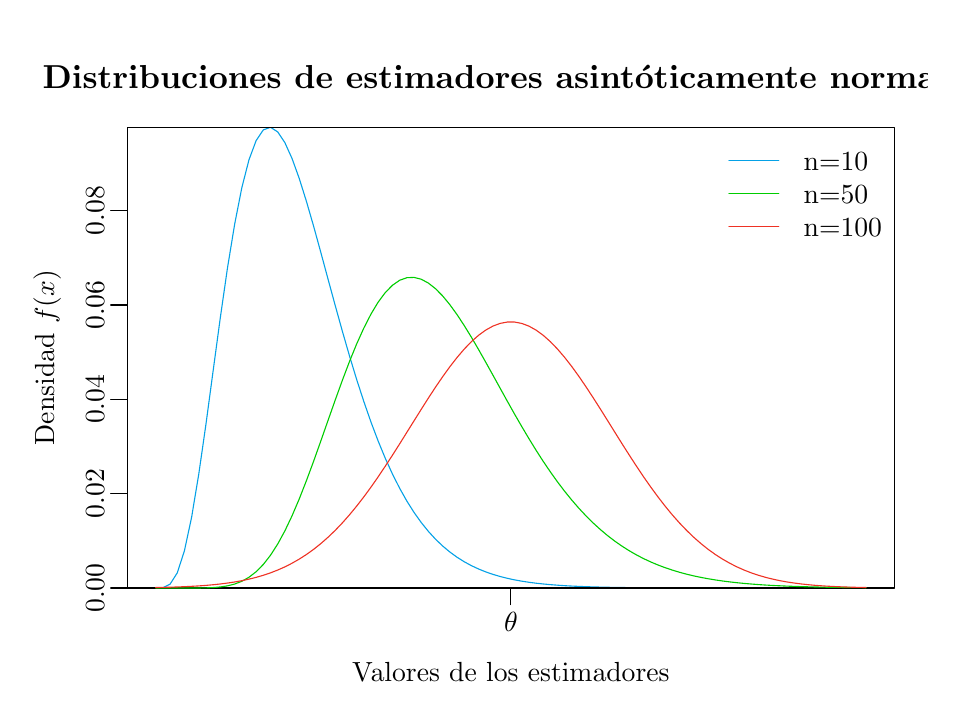
\begin{tikzpicture}[x=1pt,y=1pt]
\definecolor{fillColor}{RGB}{255,255,255}
\path[use as bounding box,fill=fillColor,fill opacity=0.00] (0,0) rectangle (325.21,238.49);
\begin{scope}
\path[clip] ( 36.00, 36.00) rectangle (313.21,202.49);
\definecolor{drawColor}{RGB}{5,161,230}

\path[draw=drawColor,line width= 0.4pt,line join=round,line cap=round] ( 46.27, 36.00) --
	( 48.86, 36.11) --
	( 51.45, 37.39) --
	( 54.05, 41.48) --
	( 56.64, 49.46) --
	( 59.23, 61.54) --
	( 61.82, 77.14) --
	( 64.42, 95.20) --
	( 67.01,114.46) --
	( 69.60,133.63) --
	( 72.19,151.59) --
	( 74.79,167.47) --
	( 77.38,180.65) --
	( 79.97,190.77) --
	( 82.57,197.72) --
	( 85.16,201.56) --
	( 87.75,202.49) --
	( 90.34,200.83) --
	( 92.94,196.94) --
	( 95.53,191.21) --
	( 98.12,184.03) --
	(100.71,175.78) --
	(103.31,166.79) --
	(105.90,157.38) --
	(108.49,147.79) --
	(111.09,138.24) --
	(113.68,128.92) --
	(116.27,119.94) --
	(118.86,111.42) --
	(121.46,103.42) --
	(124.05, 95.98) --
	(126.64, 89.13) --
	(129.23, 82.86) --
	(131.83, 77.17) --
	(134.42, 72.04) --
	(137.01, 67.44) --
	(139.61, 63.33) --
	(142.20, 59.69) --
	(144.79, 56.48) --
	(147.38, 53.65) --
	(149.98, 51.17) --
	(152.57, 49.01) --
	(155.16, 47.13) --
	(157.75, 45.50) --
	(160.35, 44.09) --
	(162.94, 42.88) --
	(165.53, 41.83) --
	(168.13, 40.94) --
	(170.72, 40.17) --
	(173.31, 39.52) --
	(175.90, 38.96) --
	(178.50, 38.49) --
	(181.09, 38.09) --
	(183.68, 37.75) --
	(186.27, 37.47) --
	(188.87, 37.23) --
	(191.46, 37.03) --
	(194.05, 36.85) --
	(196.65, 36.71) --
	(199.24, 36.59) --
	(201.83, 36.49) --
	(204.42, 36.41) --
	(207.02, 36.34) --
	(209.61, 36.28) --
	(212.20, 36.23) --
	(214.79, 36.19) --
	(217.39, 36.16) --
	(219.98, 36.13) --
	(222.57, 36.11) --
	(225.17, 36.09) --
	(227.76, 36.07) --
	(230.35, 36.06) --
	(232.94, 36.05) --
	(235.54, 36.04) --
	(238.13, 36.03) --
	(240.72, 36.03) --
	(243.31, 36.02) --
	(245.91, 36.02) --
	(248.50, 36.01) --
	(251.09, 36.01) --
	(253.69, 36.01) --
	(256.28, 36.01) --
	(258.87, 36.01) --
	(261.46, 36.01) --
	(264.06, 36.00) --
	(266.65, 36.00) --
	(269.24, 36.00) --
	(271.83, 36.00) --
	(274.43, 36.00) --
	(277.02, 36.00) --
	(279.61, 36.00) --
	(282.21, 36.00) --
	(284.80, 36.00) --
	(287.39, 36.00) --
	(289.98, 36.00) --
	(292.58, 36.00) --
	(295.17, 36.00) --
	(297.76, 36.00) --
	(300.36, 36.00) --
	(302.95, 36.00);
\end{scope}
\begin{scope}
\path[clip] (  0.00,  0.00) rectangle (325.21,238.49);
\definecolor{drawColor}{RGB}{0,0,0}

\path[draw=drawColor,line width= 0.4pt,line join=round,line cap=round] ( 36.00, 36.00) -- ( 36.00,172.38);

\path[draw=drawColor,line width= 0.4pt,line join=round,line cap=round] ( 36.00, 36.00) -- ( 30.00, 36.00);

\path[draw=drawColor,line width= 0.4pt,line join=round,line cap=round] ( 36.00, 70.09) -- ( 30.00, 70.09);

\path[draw=drawColor,line width= 0.4pt,line join=round,line cap=round] ( 36.00,104.19) -- ( 30.00,104.19);

\path[draw=drawColor,line width= 0.4pt,line join=round,line cap=round] ( 36.00,138.28) -- ( 30.00,138.28);

\path[draw=drawColor,line width= 0.4pt,line join=round,line cap=round] ( 36.00,172.38) -- ( 30.00,172.38);

\node[text=drawColor,rotate= 90.00,anchor=base,inner sep=0pt, outer sep=0pt, scale=  1.00] at ( 27.60, 36.00) {0.00};

\node[text=drawColor,rotate= 90.00,anchor=base,inner sep=0pt, outer sep=0pt, scale=  1.00] at ( 27.60, 70.09) {0.02};

\node[text=drawColor,rotate= 90.00,anchor=base,inner sep=0pt, outer sep=0pt, scale=  1.00] at ( 27.60,104.19) {0.04};

\node[text=drawColor,rotate= 90.00,anchor=base,inner sep=0pt, outer sep=0pt, scale=  1.00] at ( 27.60,138.28) {0.06};

\node[text=drawColor,rotate= 90.00,anchor=base,inner sep=0pt, outer sep=0pt, scale=  1.00] at ( 27.60,172.38) {0.08};

\path[draw=drawColor,line width= 0.4pt,line join=round,line cap=round] ( 36.00, 36.00) --
	(313.21, 36.00) --
	(313.21,202.49) --
	( 36.00,202.49) --
	( 36.00, 36.00);
\end{scope}
\begin{scope}
\path[clip] (  0.00,  0.00) rectangle (325.21,238.49);
\definecolor{drawColor}{RGB}{0,0,0}

\node[text=drawColor,anchor=base,inner sep=0pt, outer sep=0pt, scale=  1.20] at (174.61,216.35) {\bfseries Distribuciones de estimadores asintóticamente normales};

\node[text=drawColor,anchor=base,inner sep=0pt, outer sep=0pt, scale=  1.00] at (174.61,  2.40) {Valores de los estimadores};

\node[text=drawColor,rotate= 90.00,anchor=base,inner sep=0pt, outer sep=0pt, scale=  1.00] at (  9.60,119.25) {Densidad $f(x)$};
\end{scope}
\begin{scope}
\path[clip] ( 36.00, 36.00) rectangle (313.21,202.49);
\definecolor{drawColor}{RGB}{0,205,0}

\path[draw=drawColor,line width= 0.4pt,line join=round,line cap=round] ( 46.27, 36.00) --
	( 48.86, 36.00) --
	( 51.45, 36.00) --
	( 54.05, 36.00) --
	( 56.64, 36.00) --
	( 59.23, 36.01) --
	( 61.82, 36.02) --
	( 64.42, 36.07) --
	( 67.01, 36.17) --
	( 69.60, 36.39) --
	( 72.19, 36.79) --
	( 74.79, 37.44) --
	( 77.38, 38.44) --
	( 79.97, 39.90) --
	( 82.57, 41.91) --
	( 85.16, 44.54) --
	( 87.75, 47.86) --
	( 90.34, 51.89) --
	( 92.94, 56.65) --
	( 95.53, 62.10) --
	( 98.12, 68.17) --
	(100.71, 74.77) --
	(103.31, 81.78) --
	(105.90, 89.06) --
	(108.49, 96.45) --
	(111.09,103.81) --
	(113.68,110.98) --
	(116.27,117.81) --
	(118.86,124.16) --
	(121.46,129.92) --
	(124.05,134.99) --
	(126.64,139.30) --
	(129.23,142.78) --
	(131.83,145.42) --
	(134.42,147.21) --
	(137.01,148.14) --
	(139.61,148.25) --
	(142.20,147.59) --
	(144.79,146.20) --
	(147.38,144.16) --
	(149.98,141.52) --
	(152.57,138.37) --
	(155.16,134.79) --
	(157.75,130.84) --
	(160.35,126.61) --
	(162.94,122.17) --
	(165.53,117.58) --
	(168.13,112.91) --
	(170.72,108.21) --
	(173.31,103.53) --
	(175.90, 98.92) --
	(178.50, 94.42) --
	(181.09, 90.05) --
	(183.68, 85.84) --
	(186.27, 81.81) --
	(188.87, 77.98) --
	(191.46, 74.35) --
	(194.05, 70.94) --
	(196.65, 67.74) --
	(199.24, 64.76) --
	(201.83, 61.99) --
	(204.42, 59.43) --
	(207.02, 57.07) --
	(209.61, 54.90) --
	(212.20, 52.92) --
	(214.79, 51.11) --
	(217.39, 49.47) --
	(219.98, 47.98) --
	(222.57, 46.63) --
	(225.17, 45.42) --
	(227.76, 44.33) --
	(230.35, 43.35) --
	(232.94, 42.48) --
	(235.54, 41.70) --
	(238.13, 41.00) --
	(240.72, 40.38) --
	(243.31, 39.84) --
	(245.91, 39.35) --
	(248.50, 38.93) --
	(251.09, 38.55) --
	(253.69, 38.22) --
	(256.28, 37.93) --
	(258.87, 37.67) --
	(261.46, 37.45) --
	(264.06, 37.25) --
	(266.65, 37.08) --
	(269.24, 36.93) --
	(271.83, 36.81) --
	(274.43, 36.69) --
	(277.02, 36.60) --
	(279.61, 36.51) --
	(282.21, 36.44) --
	(284.80, 36.38) --
	(287.39, 36.32) --
	(289.98, 36.28) --
	(292.58, 36.24) --
	(295.17, 36.20) --
	(297.76, 36.17) --
	(300.36, 36.15) --
	(302.95, 36.12);
\definecolor{drawColor}{RGB}{238,50,36}

\path[draw=drawColor,line width= 0.4pt,line join=round,line cap=round] ( 46.27, 36.19) --
	( 48.86, 36.24) --
	( 51.45, 36.30) --
	( 54.05, 36.39) --
	( 56.64, 36.49) --
	( 59.23, 36.62) --
	( 61.82, 36.77) --
	( 64.42, 36.96) --
	( 67.01, 37.19) --
	( 69.60, 37.47) --
	( 72.19, 37.80) --
	( 74.79, 38.19) --
	( 77.38, 38.66) --
	( 79.97, 39.22) --
	( 82.57, 39.86) --
	( 85.16, 40.62) --
	( 87.75, 41.49) --
	( 90.34, 42.50) --
	( 92.94, 43.65) --
	( 95.53, 44.97) --
	( 98.12, 46.45) --
	(100.71, 48.11) --
	(103.31, 49.97) --
	(105.90, 52.04) --
	(108.49, 54.31) --
	(111.09, 56.80) --
	(113.68, 59.51) --
	(116.27, 62.44) --
	(118.86, 65.58) --
	(121.46, 68.93) --
	(124.05, 72.46) --
	(126.64, 76.17) --
	(129.23, 80.04) --
	(131.83, 84.03) --
	(134.42, 88.11) --
	(137.01, 92.26) --
	(139.61, 96.42) --
	(142.20,100.56) --
	(144.79,104.64) --
	(147.38,108.60) --
	(149.98,112.40) --
	(152.57,115.99) --
	(155.16,119.32) --
	(157.75,122.35) --
	(160.35,125.04) --
	(162.94,127.34) --
	(165.53,129.22) --
	(168.13,130.66) --
	(170.72,131.63) --
	(173.31,132.12) --
	(175.90,132.12) --
	(178.50,131.63) --
	(181.09,130.66) --
	(183.68,129.22) --
	(186.27,127.34) --
	(188.87,125.04) --
	(191.46,122.35) --
	(194.05,119.32) --
	(196.65,115.99) --
	(199.24,112.40) --
	(201.83,108.60) --
	(204.42,104.64) --
	(207.02,100.56) --
	(209.61, 96.42) --
	(212.20, 92.26) --
	(214.79, 88.11) --
	(217.39, 84.03) --
	(219.98, 80.04) --
	(222.57, 76.17) --
	(225.17, 72.46) --
	(227.76, 68.93) --
	(230.35, 65.58) --
	(232.94, 62.44) --
	(235.54, 59.51) --
	(238.13, 56.80) --
	(240.72, 54.31) --
	(243.31, 52.04) --
	(245.91, 49.97) --
	(248.50, 48.11) --
	(251.09, 46.45) --
	(253.69, 44.97) --
	(256.28, 43.65) --
	(258.87, 42.50) --
	(261.46, 41.49) --
	(264.06, 40.62) --
	(266.65, 39.86) --
	(269.24, 39.22) --
	(271.83, 38.66) --
	(274.43, 38.19) --
	(277.02, 37.80) --
	(279.61, 37.47) --
	(282.21, 37.19) --
	(284.80, 36.96) --
	(287.39, 36.77) --
	(289.98, 36.62) --
	(292.58, 36.49) --
	(295.17, 36.39) --
	(297.76, 36.30) --
	(300.36, 36.24) --
	(302.95, 36.19);
\definecolor{drawColor}{RGB}{5,161,230}

\path[draw=drawColor,line width= 0.4pt,line join=round,line cap=round] (253.39,190.49) -- (271.39,190.49);
\definecolor{drawColor}{RGB}{0,205,0}

\path[draw=drawColor,line width= 0.4pt,line join=round,line cap=round] (253.39,178.49) -- (271.39,178.49);
\definecolor{drawColor}{RGB}{238,50,36}

\path[draw=drawColor,line width= 0.4pt,line join=round,line cap=round] (253.39,166.49) -- (271.39,166.49);
\definecolor{drawColor}{RGB}{0,0,0}

\node[text=drawColor,anchor=base west,inner sep=0pt, outer sep=0pt, scale=  1.00] at (280.39,187.05) {n=10};

\node[text=drawColor,anchor=base west,inner sep=0pt, outer sep=0pt, scale=  1.00] at (280.39,175.05) {n=50};

\node[text=drawColor,anchor=base west,inner sep=0pt, outer sep=0pt, scale=  1.00] at (280.39,163.05) {n=100};
\end{scope}
\begin{scope}
\path[clip] (  0.00,  0.00) rectangle (325.21,238.49);
\definecolor{drawColor}{RGB}{0,0,0}

\path[draw=drawColor,line width= 0.4pt,line join=round,line cap=round] (174.61, 36.00) -- (174.61, 36.00);

\path[draw=drawColor,line width= 0.4pt,line join=round,line cap=round] (174.61, 36.00) -- (174.61, 30.00);

\node[text=drawColor,anchor=base,inner sep=0pt, outer sep=0pt, scale=  1.00] at (174.61, 20.40) {$\theta$};
\end{scope}
\end{tikzpicture}
